\section{Competition results\label{section:stamina-results}}

The Stamina competition started on March 2010 with the 31th of December announced as an official deadline for submitting results. Between these two dates, 1856 submissions have been made by 11 challengers. Among them, 61 have a BCR score of at least 99\%, breaking 42 different problems in 10 different cells.

The competition hall of fame is shown in Fig.\ref{table:stamina-hall-of-fame}. The easiest cell (alphabet 2, sparsity 100\%) has been quickly broken --~five days after the competition start~-- by Manuel V\'azquez de Parga Andrade with the Equipo algorithm, that learns automata teams~\cite{Garcia:2010}). This first result has been followed by an apparent lull in the competition. Some challengers were actually submitting at that time without successfully breaking new problems and cells. Therefore, in the absence of a more detailed hall of fame, this activity was not directly visible on the competition website. A few weeks after, Marijn Heule and Sicco Verwer, with the DFASAT algorithm (described later), started solving all cells of difficulty~1 in the left-most column. After a new apparent lull, they eventually broke the first cell of difficulty~2 (alphabet 50, sparsity 100\%) therefore taking the head of the competition. They eventually won the competition with an extra cell broken (alphabet 50, sparsity 50\%), the only cell of difficulty~3 broken during the competition. Individual problems have also been broken in cells of the second column (sparsity 50\%), as shown by numbers in Table~\ref{table:stamina-hall-of-fame}.

\begin{table}
\begin{center}
\begin{tabular}{c|c c c c}
&\multicolumn{4}{|c}{\textbf{Sparsity}}\\ 
\textbf{$|\Sigma|$} & \textbf{100\%} & \textbf{50\%} & \textbf{25\%} & \textbf{12.5\%}\\
\hline
\textbf{2}  & Equipo (1) & \emph{4 broken} (1)  & - (3) & - (3) \\
\textbf{5}  & DFASAT (1) & \emph{1 broken} (2)  & - (4) & - (4) \\
\textbf{10} & DFASAT (1) & \emph{3 broken} (3)  & - (4) & - (4) \\
\textbf{20} & DFASAT (1) & \emph{4 broken} (3)  & - (4) & - (4) \\
\textbf{50} & DFASAT (2) & DFASAT (3) & - (4) & - (4) \\
\end{tabular}
\end{center}
\caption{Stamina hall of fame. Broken cells are annotated with the winner name. In other cells, the number in italics indicates how many of the five problems were broken the 31th of December, if any. Difficulty levels in parenthesis are recalled from Table~\ref{table:stamina-baseline}.\label{table:stamina-hall-of-fame}}
\end{table}

The fact that DFASAT has broken the cell (alphabet 50, sparsity 50\%) but not easier cells in the same column might appear strange at first glance. This result must first be slightly weakened, then explained. First, one can verify in Table~\ref{table:stamina-hall-of-fame} that 17 of the 25 problems of the column have been actually broken (all of them are broken by DFASAT). Strategic participant choices must also be taken into account. After having solved cells of difficulty 1 and 2, they probably focused on solving cells of higher difficulty. This precaution taken, the fact that DFASAT relies on a useful scoring heuristics for large alphabets is certainly important for explaining their success on that hardest cell (see Section~\ref{subsection:stamina-winning}).

As the same table shows, no problem has been broken in the last two columns, that is with a sample sparsity of 25\% or less. Here again, this fact must be interpreted with caution. First, while fewer activity has been monitored on such cells, a few approaches actually performed quite well -- above the baseline in particular. Also, because of specific strategies used by the different participants, only partial results were available at the end of the competition. In other words, participants have not submitted results on all available problems, so that making comparisons and drawing conclusions is made difficult. Before discussing trends on those hardest cells, however, let be fair and present key ingredients used by the winning algorithm.

\subsection{The winning algorithm\label{subsection:stamina-winning}}

DFASAT reuses the baseline algorithm in an appropriate way but relies on additional key ingredients: an adapted heuristics for scoring candidate merging operations, a random perturbation of such heuristics and intense search after an original reduction to a satisfiability problem (hence the DFA\textbf{SAT} name). Each of them is described in turn in the following sections.

\subsubsection*{Regular induction seen as a SAT problem}

The idea behind the satisfiability part of DFASAT is to first reduce the problem of finding the minimal DFA consistent with a labeled sample to a graph coloring problem, to encode the latter into a satisfiability problem, and finally to solve it using an efficient SAT solver. 

The principle of reducing DFA induction to graph coloring dates back to 1997 (more or less as the Abbadingo contest itself, see e.g.~\cite{Coste:1997}) and roughly proceeds as follows. Consider an undirected graph made of one node for each state of the augmented PTA encoding the training sample. Two nodes of this graph are connected if they cannot be merged, that is, if their respective state in the PTA have different labels (i.e. accepting vs. error state) or if merging them would lead to merging states of different labels in virtue of the determinization process. These transitions can be computed in a way similar to the pre-computation of incompatibilities between PTA states which is sometimes used in classical state merging algorithms, e.g.~\cite{Coste:1998, Coste:2004}. Coloring the graph obtained with different colors for adjacent nodes is equivalent to finding a consistent DFA. Indeed, used colors defines a partition of the PTA states (see Section~\ref{section:inductive-background}) so that merging states of the same color leads to a DFA, which is consistent with the sample by construction. The amount of colors being equal to the size of the DFA, finding the minimum leads to solving the problem of minimal consistent DFA.

The main drawback of such an approach is that the number of graph nodes, and of edges capturing coloring constraints, quickly becomes huge for big samples. This can lead to coloring problem instances that are impractical in practice. In spite of a compact boolean encoding of the graph coloring problem and huge enhancements in SAT solving in recent years, some of the Abbadingo and Stamina problems remain intractable with this technique only. See~\cite{Heule:2010}, by the same authors as DFASAT, for details about their graph coloring and SAT translations.

\subsubsection*{Mixing state-merging and SAT solving}

To overcome this tractability problem, the authors reuse classical state-merging upstream their SAT solving technique. The idea here is to execute the first steps of Blue-fringe (or another EDSM variant) to first reduce the PTA to a partially identified DFA. Indeed, the SAT encoding of the authors does not depend on a tree-shaped automaton and is sufficiently flexible to work with any DFA. However, if executing even the first steps of a state-merging algorithm drastically reduce the number of states, and hence the number of constraints, this state-merging step implies that the solution provided by the SAT solver is no longer exact. Nevertheless the first few merges performed by Blue-fringe are normally supported by a lot of evidence. Consequently, they are likely to be correct and are then expected to lead to an optimal solution in practice~\cite{Heule:2010}, provided that a good scoring heuristics is used. 

Interestingly, according to the winners themselves, the EDSM + SAT technique so far was not sufficient to break Stamina cells above the first difficulty level. As another technique already had gained a cell of same difficulty they have had to further optimize their technique, as explained in the next section.

\subsubsection*{A few additional ingredients required}

In order to obtain convincing results on those harder cells, a few additional ingredients to the procedure described so far are required:

The first one is a different scoring heuristics than the one used by EDSM/Blue-fringe. Indeed, since Abbadingo it is commonly admitted that the heuristics must be based on the number of merged states sharing the same label. To win the Stamina competition, however, DFASAT had to use a different one, related to the number of merged transitions sharing the same symbol. The explanation relies on the kind of automata considered, especially on large alphabets (see Section~\ref{subsection:stamina-machines}): as two different states of the target DFA are unlikely to have many outgoing transitions in common, two PTA states having more than a few of them are very likely to correspond to the same target state.

Also, Instead of considering only one solution, as commonly done with greedy state-merging algorithms like Blue-fringe, DFASAT includes a search strategy over multiple candidates. While this is natural with SAT-based graph coloring applied to grammar induction (since all possible solutions are captured in a compact form) the authors have also intentionally introduced search in two other places. The first one involves a random perturbation of the scoring heuristics, to reduce the criticality of wrong initial merges potentially made during the first phase. The second one was to also look for non-minimal consistent automata by considering more colors than actually required for coloring the graph. While doing so appears in contradiction with the Occam's razor principle at first glance, it actually makes sense in the context of Stamina. Indeed, the actual problem to solve in the competition is not strictly speaking the identification of target automata but the learning of good approximate solutions reaching 99\% of BCR score. In view of the competition setup and generation protocols, looking for automata of about 50 states is probably a better criteria than looking for the minimal consistent one.

\subsection{Trends on hardest cells\label{subsection:stamina-trends-on-hardest-cells}}

Table~\ref{table:stamina-hall-of-fame} only reveals competition activity according to its winning criteria, that is, to be the first to break the hardest cell among those broken. Interesting hidden activity (so far) may be revealed and trends drawn if we turn to a different criteria for presenting the hall of fame. Consider the Table~\ref{table:stamina-hall-of-fame-2}. In contrast to Table~\ref{table:stamina-hall-of-fame} that considers broken cells only, this one shows for each cell the name of the best technique together with its average score on cell problems. To keep a fair comparison criteria by cell, only participants that have submitted for the five problems it contains are taken into account. Also, only the best participant score for each problem is kept for computing the average score of the cell. Last, only results above the baseline are taken into account. In other words, empty cells may be interpreted as being owned by the baseline itself. 

Results in Table~\ref{table:stamina-hall-of-fame-2} have been compiled according to that criteria, from available data at competition termination. Two observations are straightforward: 

\begin{itemize}

\item First, the pbc algorithm (\emph{pcb} stands for \emph{pattern based classification}, a modification of the technique presented in~\cite{Lo:2009}) performs well on hardest problems in comparison with the baseline which obtains around 0.52 in average for the same cells (baseline scores have been given in Table~\ref{table:stamina-baseline}). 

\item Second, DFASAT is near of breaking a cell of difficulty 4 (alphabet 50, sparsity 25\%), with an average score of 0.967. Interestingly, the variance is small (the best score being 0.985 and the worse 0.929) which supports our claim. The other score obtained on this column (0.788 on alphabet 2, sparsity 25\%) tend to confirm the usefulness of DFASAT's scoring heuristics discussed in the previous section, since better results are obtained on large alphabets than on small ones (here also, strategic choices made by DFASAT might also partly explain this difference).

\end{itemize}

\begin{table}[H]
\begin{center}
\begin{tabular}{c|c c c c}
&\multicolumn{4}{|c}{\textbf{Sparsity}}\\ 
\textbf{$|\Sigma|$} & \textbf{100\%} & \textbf{50\%} & \textbf{25\%} & \textbf{12.5\%}\\
\hline
\textbf{2}  & DFASAT (\emph{br.}) & DFASAT (0.987)      & DFASAT (0.788) &  \\
\textbf{5}  & DFASAT (\emph{br.}) & DFASAT (0.968)      &                &  \\
\textbf{10} & DFASAT (\emph{br.}) & DFASAT (0.979)      & pbc (0.680)    & pbc (0.688) \\
\textbf{20} & DFASAT (\emph{br.}) & DFASAT (0.991)      & pbc (0.734)    & pbc (0.726) \\
\textbf{50} & DFASAT (\emph{br.}) & DFASAT (\emph{br.}) & DFASAT (0.967) & pbc (0.750) \\
\end{tabular}
\end{center}
\caption{Hall of fame based on average scoring by cell, provided that the participant has submitted for all problems in the cell (\emph{br.} stands for \emph{broken}).\label{table:stamina-hall-of-fame-2}}
\end{table}

The fact that only partial results are available do not allow fully drawing comparisons between scores obtained by the different approaches. For example, pbc did not submit on smallest alphabets while DFASAT did not submit on sparsest samples, as illustrated in Fig.~\ref{image:stamina-winners-performance-comparison} where their respective performance curves are plotted. Also, a few other techniques significantly outperformed the baseline on a variety of problems, but have not submitted for all problems of a given cell and are therefore not taken into account in Table~\ref{table:stamina-hall-of-fame-2}. Even when restricting our attention to pbc and DFASAT, the table shows that, while pbc performs well, it is very likely that DFASAT would outperform it on sparsest samples. Two observations support this claim. First, cells where both algorithms have submitted are credited to DFASAT (sparsity of 50\% on largest alphabets, for instance). Also, with a sparsity of 25\%, DFASAT already outperforms pbc in average on the two cells with smallest and largest alphabets. 

\begin{figure}[ht]
\centering\scalebox{.26}{
  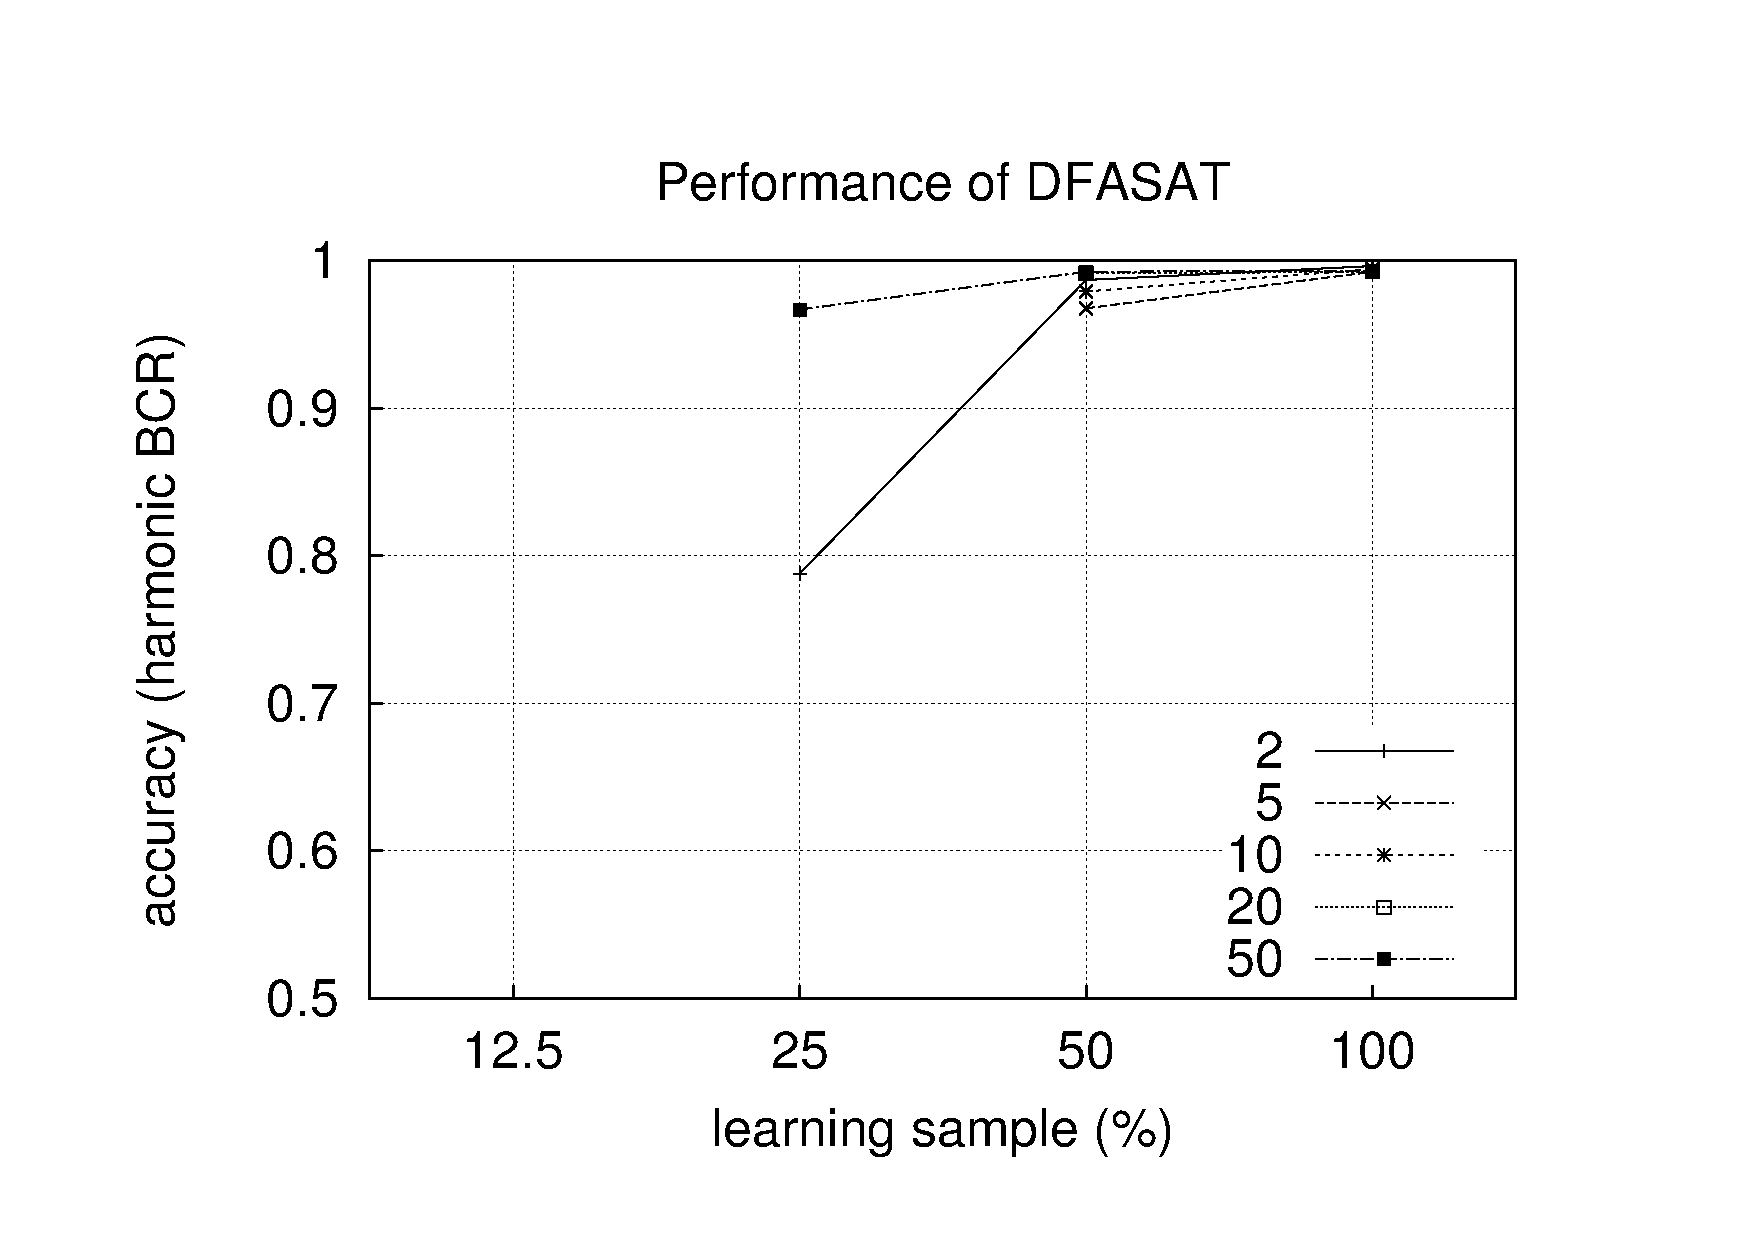
\includegraphics[trim=20mm 0mm 25mm 0mm, clip]{src/6-stamina/images/DFASAT-performance}
  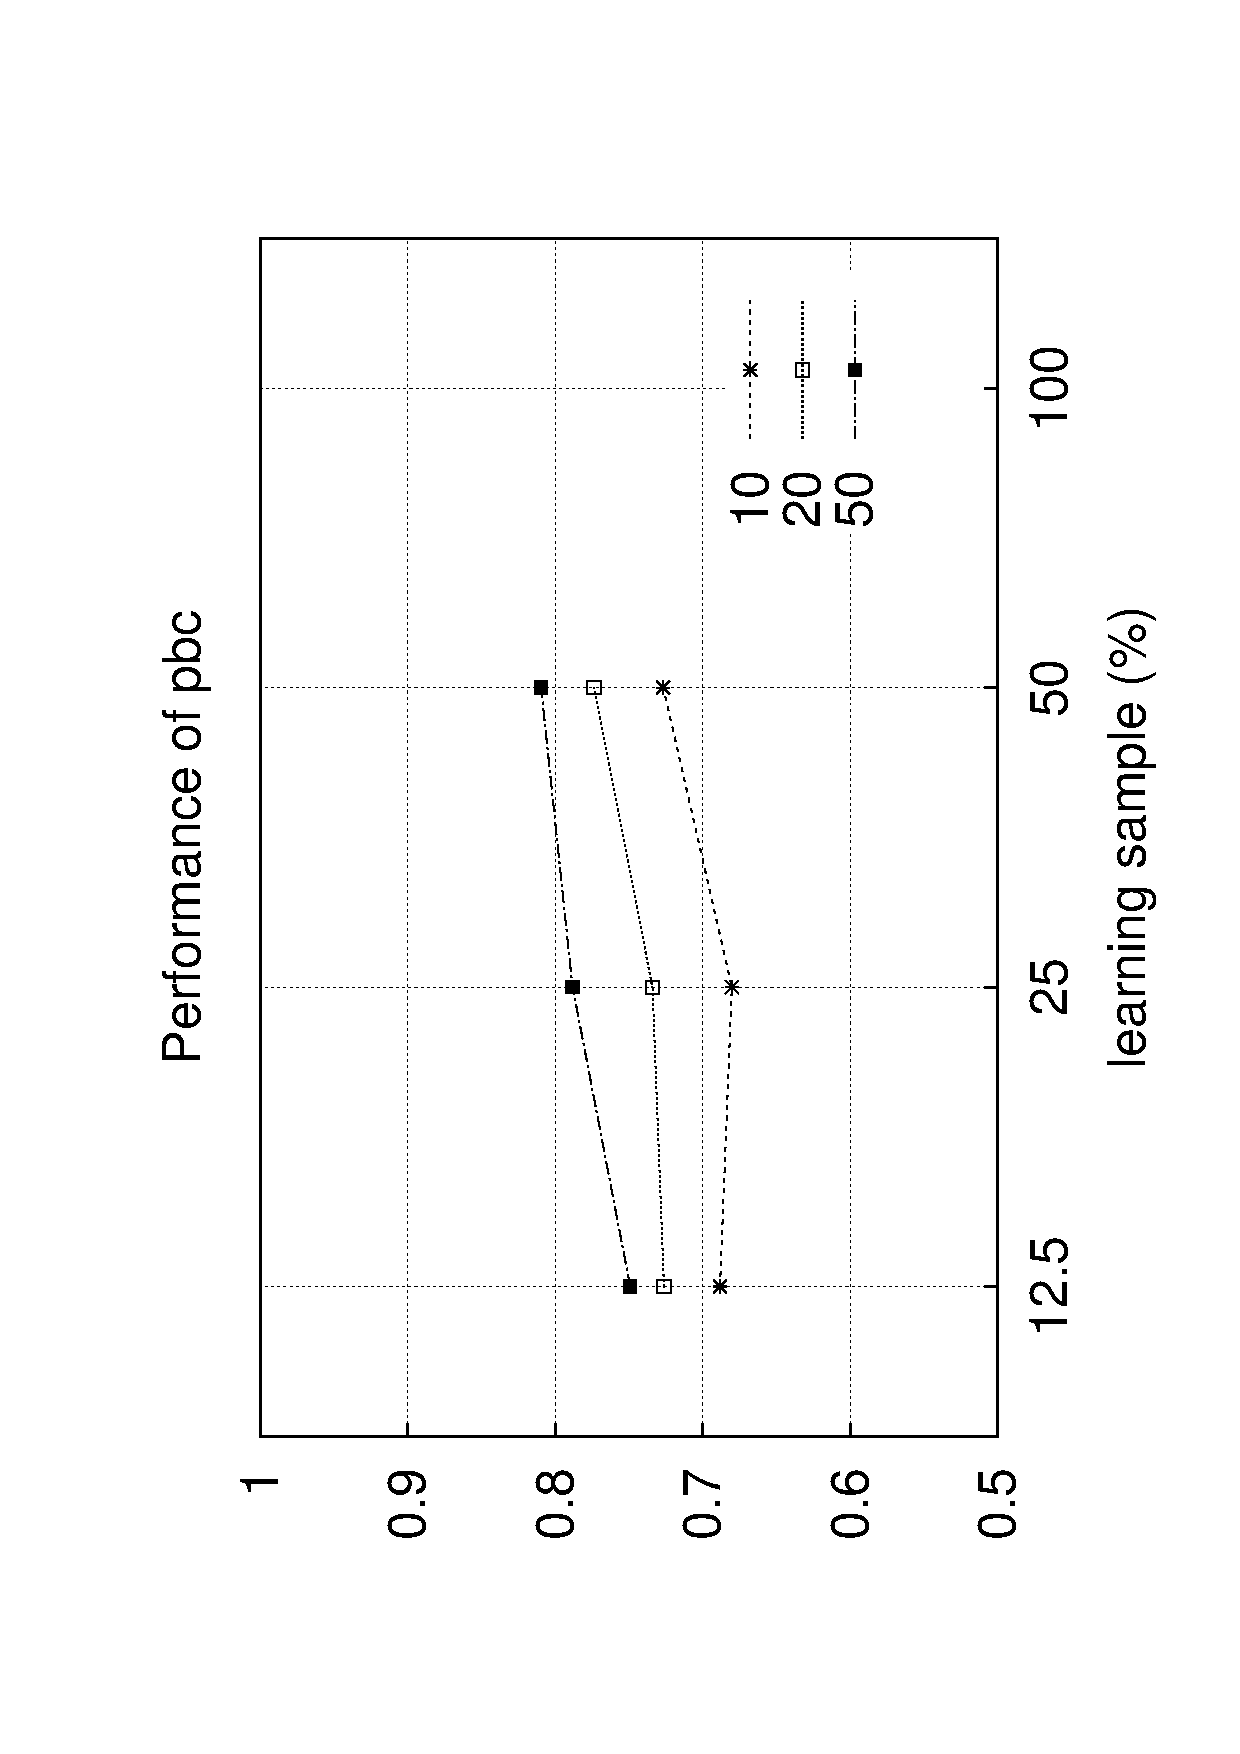
\includegraphics[trim=20mm 0mm 25mm 0mm, clip]{src/6-stamina/images/pbc-performance}}
  \caption{Performance curves of DFASAT and pbc\label{image:stamina-winners-performance-comparison}.}
\end{figure}

In any case, a quick comparison of the curves in Fig.~\ref{image:stamina-winners-performance-comparison} with the baseline curves in Fig.~\ref{stamina:image:bluefringe-performance} perfectly illustrates the overall contribution of the competition and of these two approaches in particular: on the kind of problems considered in Stamina, the state-of-the-art in grammar induction has been pushed significantly forward.

